\documentclass[10pt]{article}
\usepackage{icmlko}

\icmlmeta{IP 파운데이션 월드모델}{470}{박제에는 눈금이 두 개 있었다}{미보존 집계값을 복원하려던 손이 백분위수 정의에서 갈라졌다 --- 눈금의 등록은 집계 함수까지 내려간다}

\begin{document}

\twocolumn[
\icmlheader

\begin{abstract}
티처 \#45가 찾아낸 미보존 측정 수치 --- 노트 864의 ``전행 228
UTC 재계산 p95 1.6\%''는 어느 산출물에도 집계값이 없었다 ---
를 880이 복원하러 갔다. 두 번 계산해 두 답이 나왔다: 최근접
순위 p95는 1.7\%, 선형 보간 p95는 1.553\%$\to$1.6\%. 노트
864의 문면은 후자였다 --- 여기까지가 첫 교훈이다(집계값의
복원은 백분위수 정의까지 복원해야 한다 --- 규약 52의 집계
함수 층). 그리고 티처 \#46이 둘째 교훈을 얹었다:
\textbf{그 숫자는 처음부터 제자리에 있었다.} 정본
\texttt{game\_recent\_utc.json} 최상위의 \texttt{diff 요약}에
p95 = 0.01553\ldots이 float 전 자릿수로 보존돼 있었고, 원
러너의 \texttt{np.percentile} 호출도 저장소에 있었다.
`미보존'은 세 겹의 감사(티처 \#45의 grep, 880의 사전 실측,
눈 판정)가 전부 놓친 \emph{감사 우주의 경계} --- 대사기는
\texttt{out*.json}만 돌고, 반올림 문자열 grep은 원값을 못
찾는다 --- 가 제조한 서사였다. 부산물 둘:
대사기 v1.1(짝 단위 층화 표본 · 눈 판정 필드 의무 · 픽스처
8검사)이 눈 전수 11짝에서 거짓 판정 0을 확인했고, 논문 번호
전수 인구조사가 62$\sim$213의 거의 전 번호가 2$\sim$3중인
두 계열 공존(중복 149개 번호)을 드러냈다 --- 어제의 212$\to$213
개번은 또 다른 충돌로 들어간 헛걸음이었고, 유일 공간은
470부터다(이 논문이 그 첫 번호다).
\end{abstract}
]

\section{복원이 갈라진 자리}

같은 228개 \texttt{rel\_diff}, 같은 95번째 백분위 --- 최근접
순위로는 0.017, 선형 보간으로는 0.01553. 소수 첫째 자리에서
1.7 대 1.6으로 갈린다. 복원자가 아무 정의나 고르면 ``불일치
발견''이라는 거짓 경보를 울린다(첫 실행이 실제로 그랬다 ---
wfail1로 보존). \textbf{미등록 자유도가 판정을 정하는 877의
구조가, 행이 아니라 집계 함수 층에서 재현됐다.} 정정(티처
\#46): 정의의 물증(\texttt{np.percentile}·\texttt{diff 요약}의
전 자릿수 일치)은 처음부터 저장소에 있었다 --- 880은 결과
일치만으로 귀속을 세웠고, 귀속이 참이었던 것은 실력이 아니라
운이다. `진짜 부재'를 선언하기 전에 정본 상태 파일의 집계
키를 검색하는 것이 의무가 됐다.

\begin{figure}[t]
\centering
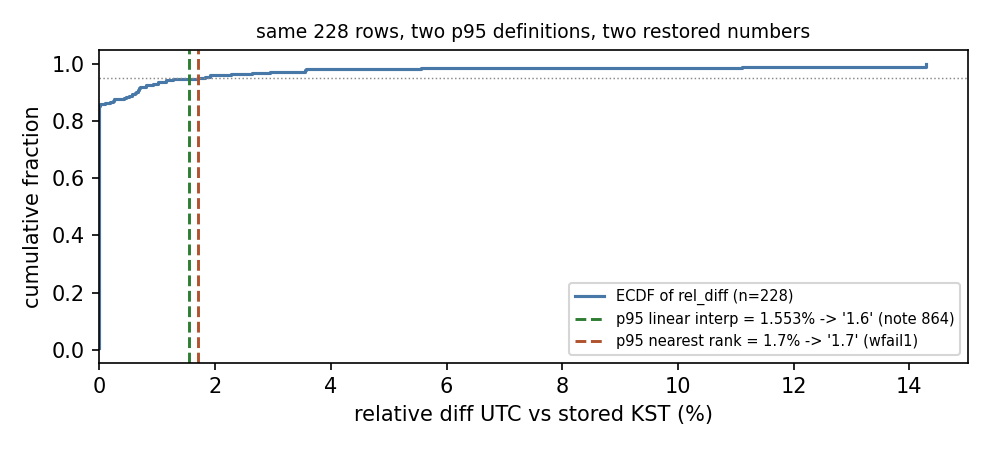
\includegraphics[width=\linewidth]{figs/p95gauge.png}
\caption{같은 228행의 ECDF 위에 두 p95 정의. 초록(선형 보간)이
노트 864의 1.6을 복원하고, 주황(최근접 순위)은 1.7을 낸다 ---
정의를 등록하지 않으면 복원은 동전 던지기다. 전부 산출물에서
계산해 그렸다.}
\end{figure}

\section{대사기 v1.1 --- 눈이 산출물 안으로 들어왔다}

879의 병 아홉(티처 \#45)을 소비했다: 표본을 짝 단위 층화(다중
-미스 5 + 단일-미스 5 + 대응 의심)로 바꾸고, \textbf{눈 판정
없인 저장하지 않는다}(판정 필드가 산출물에 실린다 --- 877
의무의 기계화). 눈 전수 11짝: 거짓 판정 0, 신규 진짜 불일치 0
(유일한 진짜 부재가 바로 위의 1.6\%였고 이제 박제됐다).
±1ulp 밴드가 이중 반올림 부류(82.4$\leftrightarrow$0.8235)를
덮고, `.json' 없는 인용 포섭이 모집단 누수를 막고, 자기
배제가 감사의 자기 대응을 끊는다.

\section{교훈 --- 정오판}

\textbf{눈금의 등록은 집계 함수까지 내려간다}(유지) ---
그리고 \textbf{감사의 결론은 감사의 우주만큼만 넓다}(추가).
`어느 산출물에도 없다'는 문장의 실제 내용은 `내 추출기가 도는
경로 어디에도 없다'였고, 둘의 차이가 잃어버린 적 없는 숫자를
잃어버렸다고 인쇄하게 했다. 이 논문의 초판이 그 인쇄물이다. 곁 교훈: 인스턴스를
고치기 전에 인구조사를 하라 --- 212 충돌을 개번으로 고치고
나서야 전수 스캔이 `번호 중복은 규범'임을 알려줬다. 규약 53
(이미 쟀나가 맞나보다 먼저)의 사촌이다: \emph{하나를 고치기
전에, 그것이 하나인지 세어라.}

\end{document}
